 \documentclass[conference]{IEEEtran}
\IEEEoverridecommandlockouts
% The preceding line is only needed to identify funding in the first footnote. If that is unneeded, please comment it out.
\usepackage{cite}
\usepackage{amsmath,amssymb,amsfonts}
\usepackage{algorithmic}
\usepackage{graphicx}
\usepackage{textcomp}
\usepackage{xcolor}
\usepackage{todonotes}

\newcommand{\Yohan}[1]{\todo[inline,backgroundcolor=green]{YC: #1}}

\def\BibTeX{{\rm B\kern-.05em{\sc i\kern-.025em b}\kern-.08em
    T\kern-.1667em\lower.7ex\hbox{E}\kern-.125emX}}
\begin{document}

\title{Numerical precision, classification accuracy, and memory footprint in the Mondrian Forest\\
\thanks{Big Data Infrastructures for Neuroinformatics Lab}
}

\author{Marc Vicuna, Martin Khannouz, Yohan Chatelain, Tristan Glatard\\
Department of Computer Science and Software Engineering\\
Concordia University, Montreal, Canada\\
first.last@concordia.ca}
% unsure if what names I should put on the paper.
%\and
%\IEEEauthorblockN{2\textsuperscript{nd} Given Name Surname}
%\IEEEauthorblockA{\textit{dept. name of organization (of Aff.)} \\
%\textit{name of organization (of Aff.)}\\
%City, Country \\
%email address or ORCID}


\maketitle

\begin{abstract}
    Randoms forests are widely used for classification and regression tasks in machine learning, but lacks delayed labelling and distributability in low power and low memory environments. The Mondrian forest, a variant of random forests based on Mondrian processes, attempts to solves these issues. However, its current implementations suffers from a still too large memory footprint for its intended use: connected devices.  This issue can largely be attributed to the use of double precision for the node bounds.  Focusing on the use case of Human Activity Recognition, we explore reduced floating-point representations of the OrpailleCC implementation of the Mondrian forest to find realistic memory reductions without significant loss in F1 score. Results show the memory occupied by tree nodes can be reduced from 64 bits to 8 bits with same or better (4\%) F1 score. Moreover, an alternative instrumentation reducing all double precision floating-point numbers from 64 bits to 9-10 bits improves significantly and consistently the F1 score, up to an \Yohan{is it true? Wasn't it due to a bug?} improvement of 81.3\% on the Recofit dataset. 
    Thus, reducing the memory footprint of Mondrian forests is possible and can even improve the results of the current implementation. 
    Further research is needed to determine if precision tuning can be an efficient part of hyperparameter search for more machine learning models similar to the Mondrian forest.
\end{abstract}

\begin{IEEEkeywords}
numerical precision, memory footprint, Verificarlo, Mondrian, human activity recognition, data streams, classification, classification accuracy, floating-point representation
\end{IEEEkeywords}

\section{Introduction}
Random forests have now matured to a highly efficient and refined automatic tool in machine learning due to its accuracy, scalability and robustness in many real-world classification tasks. One major exception is machine learning on connected devices, such as wearable devices and other smart objects, for which random forests are too expensive in memory to train on a single device. In the attempt to make on-chip classification feasible on connected devices, adapted algorithms are needed. Online classifiers, such as the Mondrian forest, the Micro-Cluster Nearest Neighbor, the Hoeffding Tree and simple Feedforward Neural Networks, aim at training an efficient classifier in a decentralized way, distributing the training among a network of connected devices. Recent research~\cite{khannouz2020benchmark} focusing on the use case of Human Activity Recognition indicates Mondrian forests is one of the best solutions in terms of accuracy, but its memory footprint is too large for on-chip classification. Using reduced floating-point formats, we analyse the number of bits required by all floating points numbers in the OrpailleCC implementation of Mondrian forests focusing on the use case of Human Activity Recognition. Since great reduction to precision does not reduce the F1 score significantly, we encourage future optimizations to reduce the memory footprint using much smaller memory formats for bounds, thus, removing the last hurdle to making Mondrian forest on-chip classification training possible.

\section{Context}
\subsection{Float-point number formats}
\Yohan{Not only, removing LSBs has not the same impact as removing bits in the exponent}.
Since the length of the mantissa (precision) is the largest part of a double, we focus on its reduction. With one bit for the sign, we consider the minimum precision and exponent give the smallest possible memory format in bits:
\begin{equation}
\gamma=p+e+1\label{eq}
\end{equation}
where $\gamma$ is the minimum format size, \textit{p} is the precision and \textit{e} the exponent length. $\gamma$ indicates if the model can be reduced to smaller more efficient formats of the corresponding size. \cite{chatelain2019automatic} In the case of 8 bits, alternative formats to IEEE need to used, such as Microsoft’s MSFP8-11. \cite{chung2018serving} In the case of variable length floats, many models could be used, one of which is universal numbers (unum). \cite{gustafson2017beating}.
\subsection{Mondrian Forests: Efficient Online Random Forests}
The Mondrian forest is called Mondrian due to the Mondrian process underlying each tree structure of the classifier (Mondrian tree). For the purposes of this paper, its essential characteristics are that the classifier approaches the accuracy of batch random forests, is online (training can be done on multiple connected devices), is highly scalable and allows delayed labelling. \cite{b1} Mondrian forests are not adapted to high dimensional data, but since human activity recognition is in generally low-dimensional, Mondrian forests are highly adapted to data streaming with human activity on smart devices.
\subsection{A Benchmark of Data Stream Classification for Human Activity Recognition on Connected Objects}
The paper \cite{khannouz2020benchmark} evaluates data stream classifiers (Hoeffding Tree, Mondrian forest, Naïve Bayes, Feedforward Neural Network, Micro Cluster Nearest Neighbor) from the perspective of connected devices, focusing on the use case of Human Activity Recognition. It serves as a baseline for this research, both in terms of implementation and of results.  Classification performance and resource consumption (runtime, memory, and power) are measured over five datasets. The results show the Mondrian forest and Hoeffding Tree have the best performance with no difference in power consumption. However, they are too memory intensive. These insights indicate memory footprint reduction of Mondrian forests may make it the best state-of-the-art online data stream classifier.
\subsection{Verificarlo: checking floating point accuracy through Monte Carlo Arithmetic}
This research heavily relies on the numerical accuracy analysis tool Verificarlo for testing on reduced floating-point formats. Verificarlo is a “compiler tool to assess the uncertainties on a scientific code due to the floating point arithmetic” \cite{denis2016verificarlo}. Indeed, contrary to classical arithmetic, computations are limited by their floating-point format and round to the highest available precision on any operation, removing for example associativity of addition and multiplication. For our purposes, we emphasize Verificarlo can simulate the rounding and thresholding error for any exponent and mantissa precision bit-wise on any variables of code in C++.
\section{Related work}
\subsection{Fast and Efficient Bit-Level Precision Tuning}
This work in \cite{adje2021fast} proposes bit-level precision tuning, which for our proposes is synonymous to tuning of reduced floating-point representations, through generation and resolution of Integer Linear Problems (ILP) instead of iterative methods. While this approach may not be adapted for exploration of the behaviors latent to precision reduction, it serves as an alternative approach that should be considered for implementation, especially if on-the-fly precision tuning becomes necessary.
\subsection{Automatic Exploration of Reduced Floating-Point Representations in Iterative Methods}
Verificarlo is an extension to the LLVM compiler to automatically use Monte Carlo Arithmetic (MCA) \cite{denis2016verificarlo}. While MCA aims at verifying the numerical stability of a process, the VPREC backend automatically emulates any IEEE-754 floating-point operation in lower precision deterministically, for example, simulating accurately the change from double to single precision. Research in \cite{chatelain2019automatic} demonstrates its effectiveness on YALES2, a large Combustion-CFDHPC code, by achieving 28\% to 67\% reduction in communication volume by lowering precision. This same iterative approach is used in this research, for the purpose of making relevant tests tailored to the process of reducing memory footprint of the Mondrian forest for Human Activity Recognition tasks.
\section{Method}

This research consists of testing Mondrian forest classifiers across multiple dimensions, with the purpose of reducing the memory footprint used by the classifiers and of isolating the observations to a single dimension. Here is a summary of the dimensions considered.
\begin{itemize}
\item Datasets: Banos et al. (7 randomized order versions) and Recofit.
\item Random seeds: 30 different random seeds, average taken.
\item Instrumentations: ‘node’ and ‘whole’.
\item Mondrian forest classifiers: 1, 5, 10 and 50 trees.
\item Precisions (mantissa length): 1 to 52.
\item Exponent length: 2 to 11.
\end{itemize}
%This makes a total of 998 400 classifiers trained, with their accuracy and F1 score measured across training inputs. 
\subsection{Datasets}
\subsubsection{Banos et al.}
The Banos et al. dataset \cite{banos2012benchmark,banos2014dealing} is a human activity dataset with 17 participants and 9 sensors per participant. Each sensor samples a 3D acceleration, gyroscope, and magnetic field, as well as the orientation in a quaternion format, producing a total of 13 values. Sensors are sampled at 50 Hz, and each sample is associated with one of 33 activities. In addition to the 33 activities, an extra activity labeled 0 indicates no specific activity. The Banos et al. dataset is pre-processed using non-overlapping windows of one second (50 samples), and using only the 6 axes (acceleration and gyroscope) of the right forearm sensor. We compute the average and the standard deviation over the window as features for each axis. We assign the most frequent label to the window. To ensure the order of the dataset is irrelevant to our results, 7 variants of the order of this processed dataset are tested.
\subsubsection{Recofit}
The Recofit \cite{morris2014recofit} dataset is a human activity dataset containing 94 participants. Similar to the Banos et al. dataset, the activity labeled 0 indicates no specific activity. Since many activities are similar, some of them are merged. We pre-processed the dataset similarly to the Banos et al. one, using non-overlapping windows of one second, and only using 6 axes (acceleration and gyroscope) from one sensor. From these 6 axes, we used the average and the standard deviation over the window as features. F1-scores are globally much lower in this dataset, as the higher number of participants and labels make classification much harder.
\subsection{Mondrian Forest}
Each tree in a Mondrian Forest recursively splits the feature space, similar to a regular decision tree. However, the feature used in the split and its value are picked randomly. The probability to select a feature is proportional to its normalized range, and the value for the split is uniformly selected in the feature's range. \par
In OrpailleCC, the amount of memory allocated to the forest is predefined and shared by all the trees in the forest, leading to a constrained memory footprint. Thus, the memory-bounded classifier can adjust to memory limitations, for instance, by stopping tree growth or replacing existing nodes with new ones. Mondrian trees are tuned using three parameters: base count, discount factor, and budget. The base count is used to initialize the prediction for the root. The discount factor influences the nodes on how much they should use their parent prediction. \cite{khannouz2020benchmark} Finally, the budget controls the tree depth. The hyperparameters used for Mondrian forests are shown here. 
\begin{table}[htbp]
\caption{Hyperparameters used for the classifiers}
\begin{center}
\begin{tabular}{|c|c|c|c|}
\hline
\textbf{Number of trees} & \textbf{Base count}& \textbf{Discount}& \textbf{Budget} \\
\hline
\textbf{1} & 0.0 & 1.0 & 1.0\\
\textbf{5} & 0.0 & 1.0 & 0.4\\
\textbf{10} & 0.0 & 1.0 & 0.4\\
\textbf{50} & 0.0 & 1.0 & 0.2\\
\hline
\end{tabular}
\label{tab1}
\end{center}
\end{table}
Moreover, considering the memory is shared among all trees, a greater number of trees may not necessarily imply better performance: as previous research \cite{khannouz2020benchmark} shows as well as our results, the Mondrian forests with 5 and 10 trees are better than with 1 and 50. In this research, each Mondrian forest is allocated either 600 KB, 1200 KB or 3 MB of memory.\footnote{For reference, 600 KB and 3 MB correspond to RAM 1.0 and RAM 5.0 in the previous benchmark \cite{khannouz2020benchmark}}
\subsection{Instrumentation variations}
Two major approaches were taken for instrumenting Verificarlo on Mondrian trees. 
The first instrumentation (node) has the goal of analysing memory reduction on nodes of Mondrian trees. Since the attributes of the nodes composing each tree occupy approximately half of the memory allocated, reducing the precision of those attributes is a major gain in memory without compromising other operations.
The second instrumentation (whole) has the goal of analysing the impact of precision reduction on all floating-point numbers on F1 score. Here, almost every double-precision floating-point number is instrumented: the node bounds, the discount factor and budget hyperparameters and the random splits formed. This implementation considers systems where all floats have single or lower precision, allowing for an even smaller memory footprint with more involved implementation. 
To ensure the correctness of the results, both instrumentations exclude numbers used to evaluate performance from instrumentation. From this point forward, we refer to these two instrumentations as node and whole.
\subsection{Verificarlo backend}
In this experiment, we chose to use the VPREC backend of the Verificarlo tool. Indeed, our goal is to accurately simulate environments where lower precision float formats are used. As shown in Automatic Exploration of Reduced Floating-Point Representations in Iterative Methods \cite{chatelain2019automatic}, this goal corresponds to a deterministic simulation of rounding error, making the VPREC backend significantly more realistic than other Verificarlo backends for the purpose of simulating low memory floating-point number formats.
\subsection{Precision}
Our main focus is the reduction of memory footprint through reduction of the IEEE 754 double-precision floating-point format, as no single precision floating-point numbers are used in the OrpailleCC implementation of the Mondrian forest. For this experience, all models are tested on all 52 levels of precision.
\subsection{Exponents}
As explained previously, exponent length reduction is also an essential part of the memory reduction problem. We tested all exponents from 2 to 11. However, we were unable to fully test the exponent 2 and 3 models on the whole instrumentation, as reducing some hyperparameters so much would cause issues in convergence of the algorithm itself.
\subsection{Evaluation}
The main metric used in this context is the F1 score. The accuracy was also considered and is shown in the documentation, but both Banos and Recofit datasets are unbalanced, thus the F1 score is a much more adapted measure. More precisely, we analyse the F1 score itself, the F1 score difference compared to the highest precision and the F1 score deviation. The analysis of these measures ensures significant and repeatable results. Note the evaluation is explicitly excluded from both the node and whole instrumentations.
\subsection{Reproducibility}
These results can be reproduced using the README on the GitHub of this project, as well as the Docker image of the benchmark. To access the plots, only unzip the results file of the result branch.

\section{Results}
This section presents the different obtained through this benchmark. In each relevant dimension, we examine the effect of lower precision on the mantissa of double-precision integers in the OrpailleCC implementation of Mondrian forests. Unless specified otherwise, we assume exponent length 11. Table \ref{tab2} presents the relative percentage of F1-score where the final F1-score of the classifier is divided by the same corresponding classifier at full precision (52):
\begin{equation}
Gain = F1_{p=i} / F1_{p=52}-1 \label{eq3}
\end{equation}
The focus is the loss of performance depending on the precision used. Notable results are observed in later paragraphs.

\begin{table}[htbp]
\begin{minipage}{\linewidth}
\caption{Performance on precision}
\begin{center}
\resizebox{\linewidth}{!}{
\begin{tabular}{|c|c|c|c|c|c|c|c|c|c|}
\hline
\textbf{Ins}&\textbf{Data}&\textbf{Mem}&\textbf{Tr}&\textbf{1}&\textbf{2}&\textbf{3}&\textbf{4}&\textbf{5}&\textbf{6}\\
\hline
Node&Bano&0.6&1&-11.71&-3.00&2.70&3.32&3.06&3.04\\
\cline{4-10}&&&5&-0.60&1.61&1.81&-1.20&0.34&0.13\\
\cline{4-10}&&&10&-1.29&-0.20&-0.25&0.23&0.12&-0.41 \\
\cline{4-10}&&&50&-1.92&-0.65&-1.00&-0.71&-0.15&-0.38 \\
\cline{3-10}&&1.2&1&-11.75&-5.73&-1.73&-2.39&-0.46&-0.41 \\
\cline{4-10}&&&5&-4.67&-2.16&-0.07&-0.74&0.21&-0.42 \\
\cline{4-10}&&&10&-2.59&-0.51&-0.83&0.36&0.69&-0.50 \\
\cline{4-10}&&&50&-0.73&0.16&-0.14&0.17&0.29&0.57 \\
\cline{3-10}&&3.0&1&-14.55&-6.79&-1.22&-1.48&0.08&0.12 \\
\cline{4-10}&&&5&-4.02&-0.94&0.58&-0.35&0.57&0.27 \\
\cline{4-10}&&&10&-2.40&0.06&0.02&0.65&0.22&0.45 \\
\cline{4-10}&&&50&-0.59&0.39&-0.12&-0.19&0.06&0.21 \\
\cline{2-10}&Reco&0.6&1&-3.44&-1.81&-0.52&-1.84&-0.19&-1.32 \\
\cline{4-10}&&&5&-1.53&0.17&0.01&-0.81&-0.83&-1.24 \\
\cline{4-10}&&&10&0.60&1.36&0.50&0.19&1.12&0.88 \\
\cline{4-10}&&&50&3.30&1.06&0.95&0.61&1.45&0.14 \\
\cline{3-10}&&1.2&1&-7.58&-2.53&-0.60&-0.68&-1.25&-0.59 \\
\cline{4-10}&&&5&-1.69&-0.57&-0.13&-0.22&-0.39&0.08 \\
\cline{4-10}&&&10&-0.35&1.58&1.47&0.65&1.67&0.66 \\
\cline{4-10}&&&50&2.35&-0.74&0.20&-1.35&0.07&-0.72 \\
\cline{3-10}&&3.0&1&-6.39&-3.28&-0.30&-0.23&-0.24&-0.12 \\
\cline{4-10}&&&5&-1.55&-0.05&0.80&-0.06&0.29&-0.18 \\
\cline{4-10}&&&10&-1.30&0.93&0.63&-0.34&0.59&0.01 \\
\cline{4-10}&&&50&0.64&0.07&-0.39&-0.23&0.33&-0.98 \\
%I AM STILL WAITING FOR THE WHOLE RESULTS, SHOULD NOT BE LONG NOW. ALL THE CODE TO ANALYSE IT IS READY. THIS IS A COPY OF NODE RESULTS
\hline
Whole&Bano&0.6&1&-11.71&-3.00&2.70&3.32&3.06&3.04\\
\cline{4-10}&&&5&-0.60&1.61&1.81&-1.20&0.34&0.13\\
\cline{4-10}&&&10&-1.29&-0.20&-0.25&0.23&0.12&-0.41 \\
\cline{4-10}&&&50&-1.92&-0.65&-1.00&-0.71&-0.15&-0.38 \\
\cline{3-10}&&1.2&1&-11.75&-5.73&-1.73&-2.39&-0.46&-0.41 \\
\cline{4-10}&&&5&-4.67&-2.16&-0.07&-0.74&0.21&-0.42 \\
\cline{4-10}&&&10&-2.59&-0.51&-0.83&0.36&0.69&-0.50 \\
\cline{4-10}&&&50&-0.73&0.16&-0.14&0.17&0.29&0.57 \\
\cline{3-10}&&3.0&1&-14.55&-6.79&-1.22&-1.48&0.08&0.12 \\
\cline{4-10}&&&5&-4.02&-0.94&0.58&-0.35&0.57&0.27 \\
\cline{4-10}&&&10&-2.40&0.06&0.02&0.65&0.22&0.45 \\
\cline{4-10}&&&50&-0.59&0.39&-0.12&-0.19&0.06&0.21 \\
\cline{2-10}&Reco&0.6&1&-3.44&-1.81&-0.52&-1.84&-0.19&-1.32 \\
\cline{4-10}&&&5&-1.53&0.17&0.01&-0.81&-0.83&-1.24 \\
\cline{4-10}&&&10&0.60&1.36&0.50&0.19&1.12&0.88 \\
\cline{4-10}&&&50&3.30&1.06&0.95&0.61&1.45&0.14 \\
\cline{3-10}&&1.2&1&-7.58&-2.53&-0.60&-0.68&-1.25&-0.59 \\
\cline{4-10}&&&5&-1.69&-0.57&-0.13&-0.22&-0.39&0.08 \\
\cline{4-10}&&&10&-0.35&1.58&1.47&0.65&1.67&0.66 \\
\cline{4-10}&&&50&2.35&-0.74&0.20&-1.35&0.07&-0.72 \\
\cline{3-10}&&3.0&1&-6.39&-3.28&-0.30&-0.23&-0.24&-0.12 \\
\cline{4-10}&&&5&-1.55&-0.05&0.80&-0.06&0.29&-0.18 \\
\cline{4-10}&&&10&-1.30&0.93&0.63&-0.34&0.59&0.01 \\
\cline{4-10}&&&50&0.64&0.07&-0.39&-0.23&0.33&-0.98 \\
\hline
\end{tabular}
}
\label{tab2}
\end{center}
\end{minipage}
\end{table}
Figure \ref{legend} shows the legend of used for our graphs. The data examined is 4 dimensional. Points vary across number of elements used to train (x-axis), a measure of success (y-axis), the precision used (color) and the model used (line type). Since all precisions get very similar results up until the precision 9, higher precisions are in similar shades.
For simple F1 score graphs, the black line is the results of the offline classifier of reference, in this case an offline K-Nearest-Neighbors classifier (offline-KNN).
\begin{figure}[htbp]
\centerline{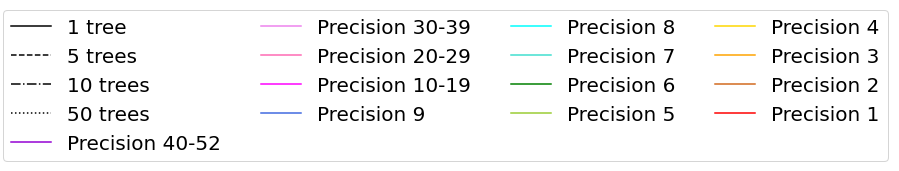
\includegraphics[width=\linewidth]{legend2.png}}
\caption{Legend for following graphs.}
\label{legend}
\end{figure}
\subsection{Instrumentations}
Figures \ref{difnode} and \ref{difwhole} are evaluations of F1 score difference on the Banos 6 dataset, where the focus is comparing instrumentations. 
\begin{figure}[htbp]
\centerline{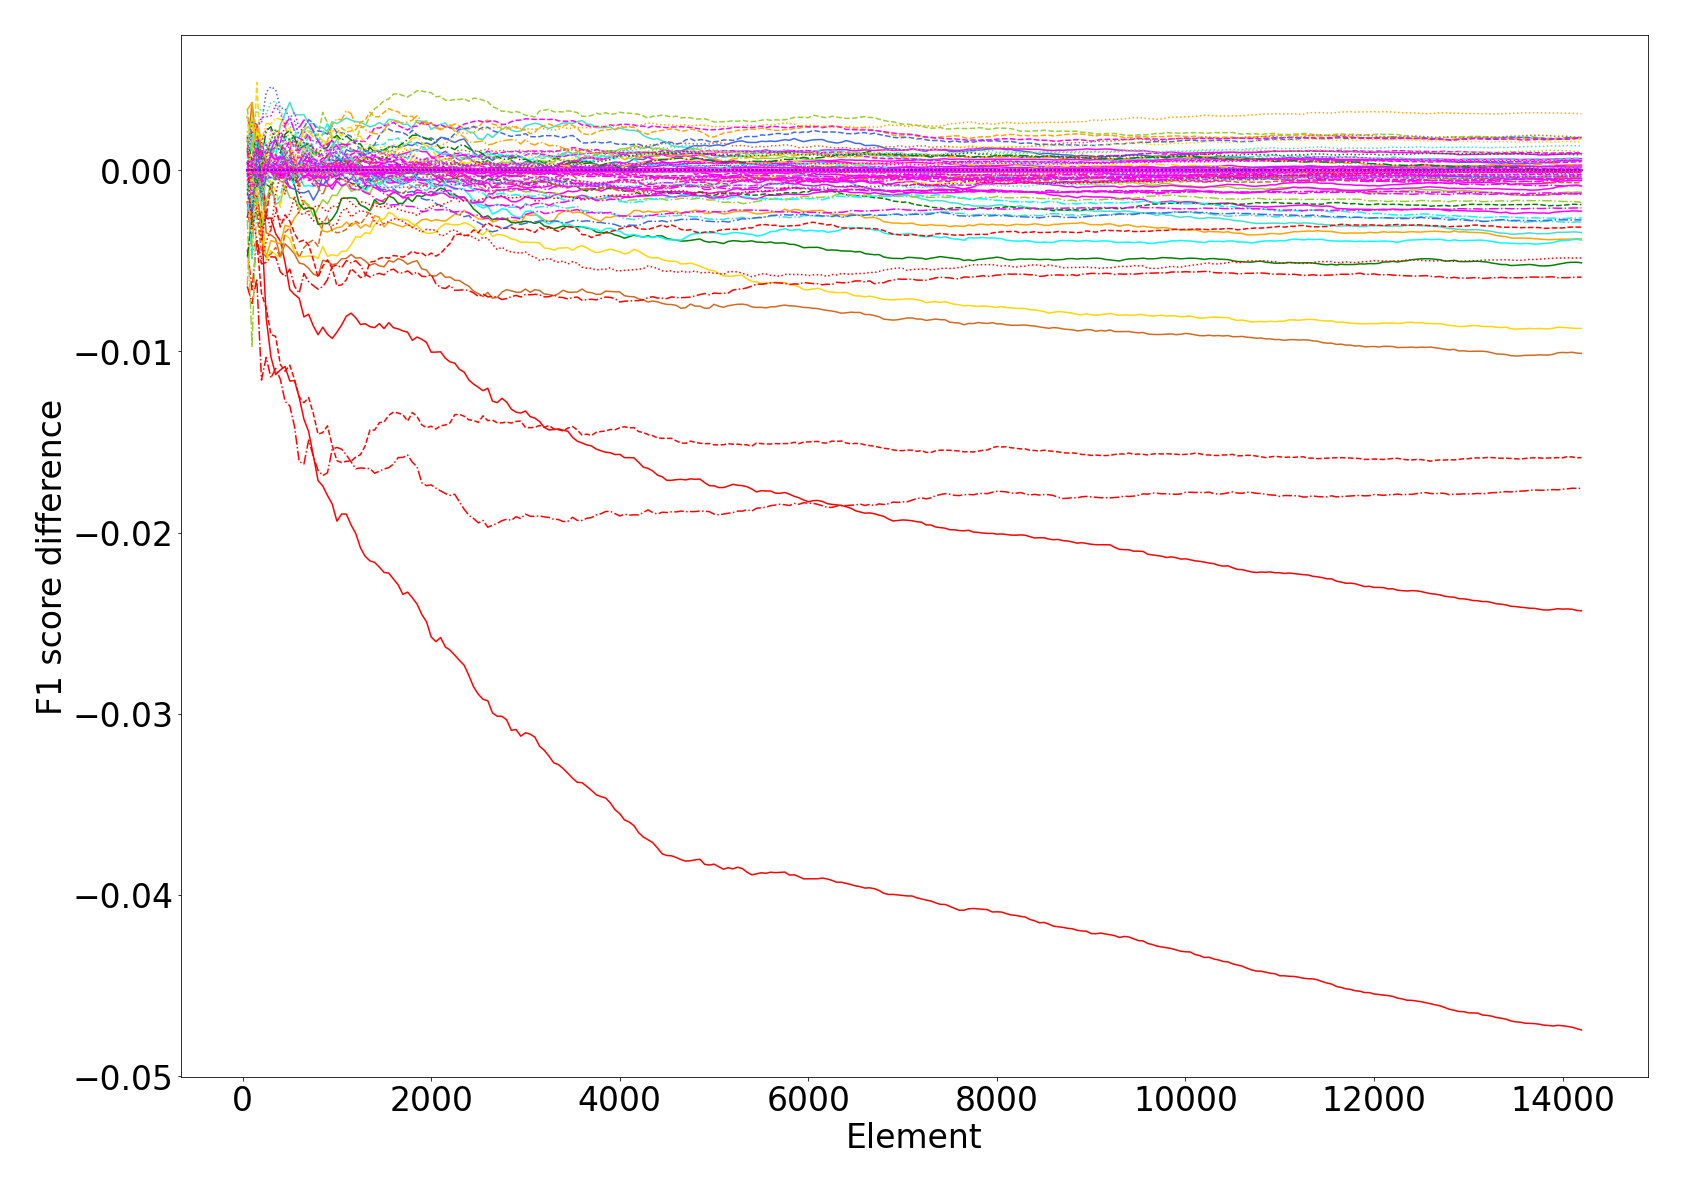
\includegraphics[width=\linewidth]{difnode11.png}}
\caption{F1 Score difference in node instrumentation between the F1 score of a precision k and the F1 score of the same model at double precision (52) and 3.0 MB. Thus, if the line is above 0, it is better than the same model at full precision, and if the line is below 0, it is worse than the same model at full precision.}
\label{difnode}
\end{figure}
\begin{figure}[htbp]
\centerline{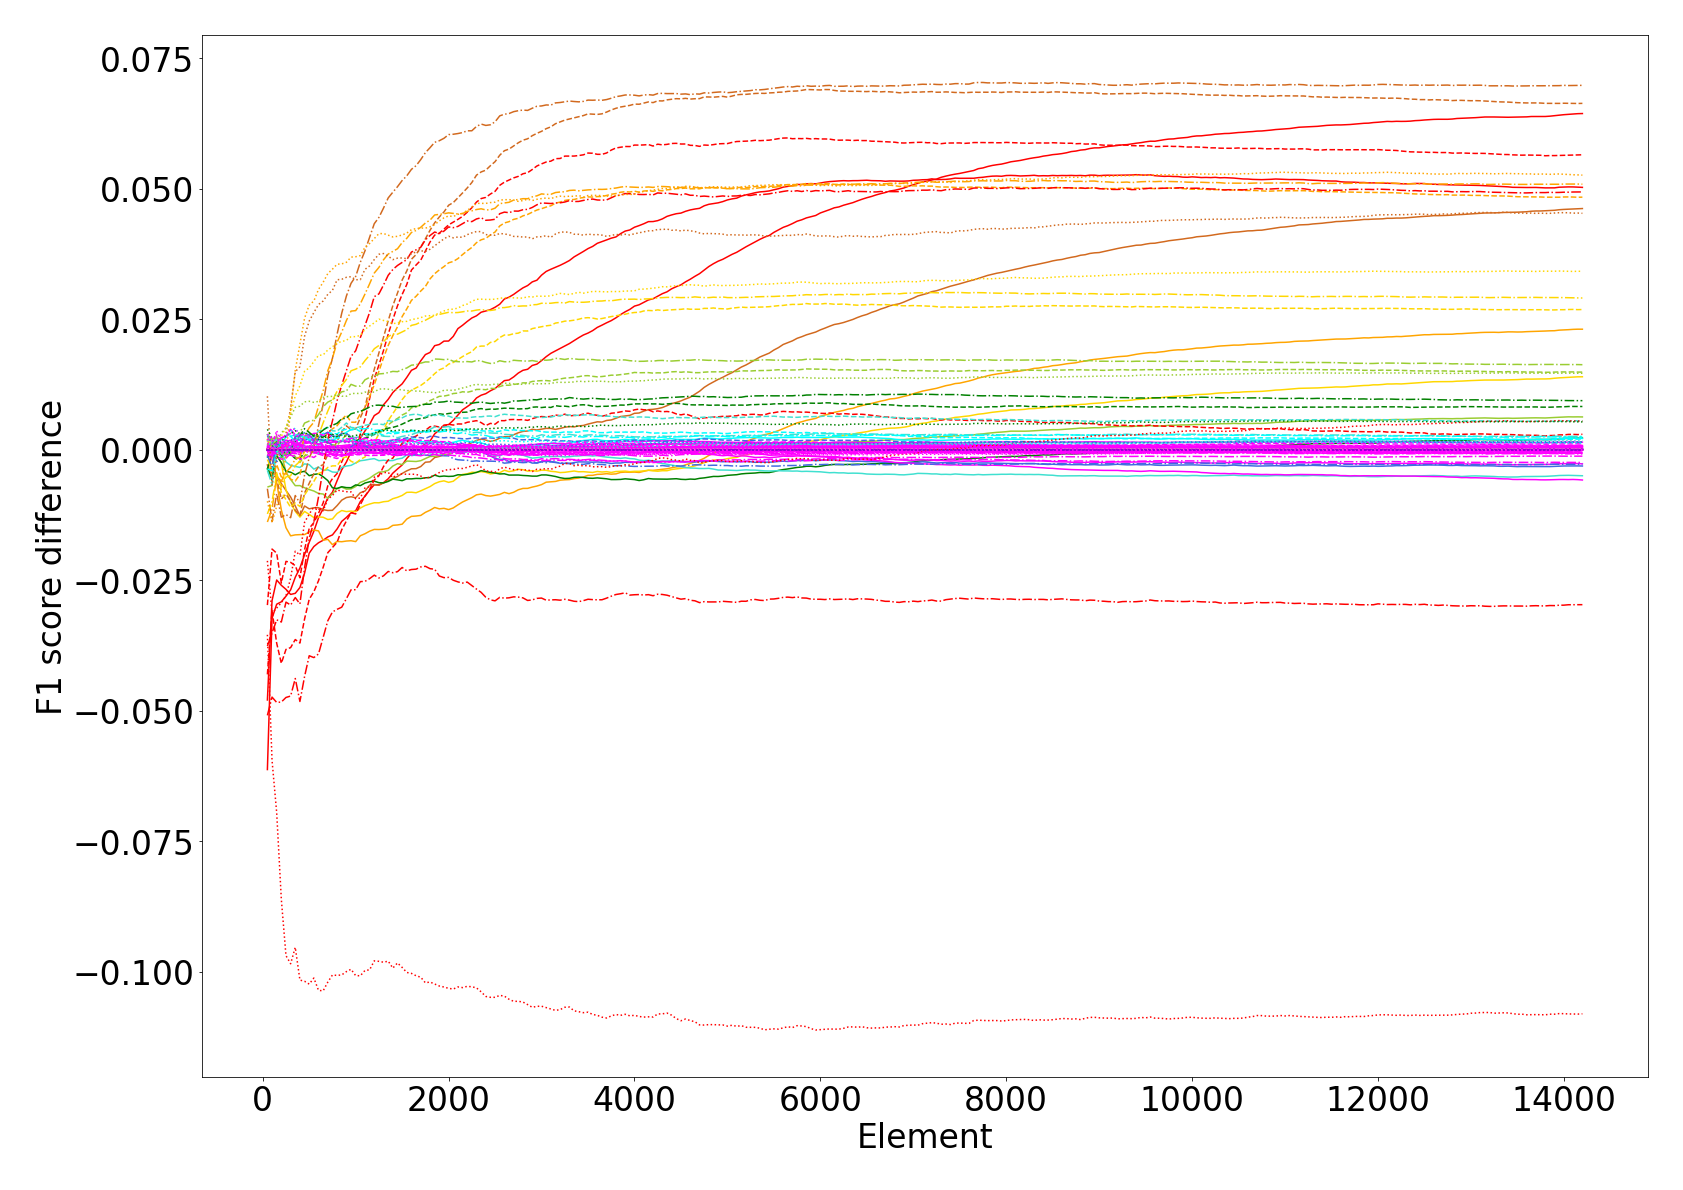
\includegraphics[width=\linewidth]{difwhole11.png}}
\caption{F1 Score difference in whole instrumentation between the F1 score of a precision k and the F1 score of the same model at double precision and 3.0 MB.}
\label{difwhole}
\end{figure}
Figure \ref{difnode} and across all results obtained and all dimensions considered, the node instrumented classifiers lose F1 score performance as precision of the mantissa is lowered. We observe in Figure \ref{difwhole} the opposite tendency in the case of the whole implementation, where the whole-instrumented classifiers gain F1 score performance as the precision is lowered, with the exception of precision 2, where the precision is too low for accurate classification. Considering the standard deviation for both instrumentations and all precisions is between 0.02 and 0.03, the variations in F1 score in the node instrumentation (excluding precision 1) are not significant, while the changes in F1 score in the whole instrumentation (precisions 1,2,3,4) are significant. Those tendencies are observed through both datasets. 
Figure 4 is the evaluation of the F1 score on the whole instrumentation, on the Recofit dataset.
\begin{figure}[htbp]
\centerline{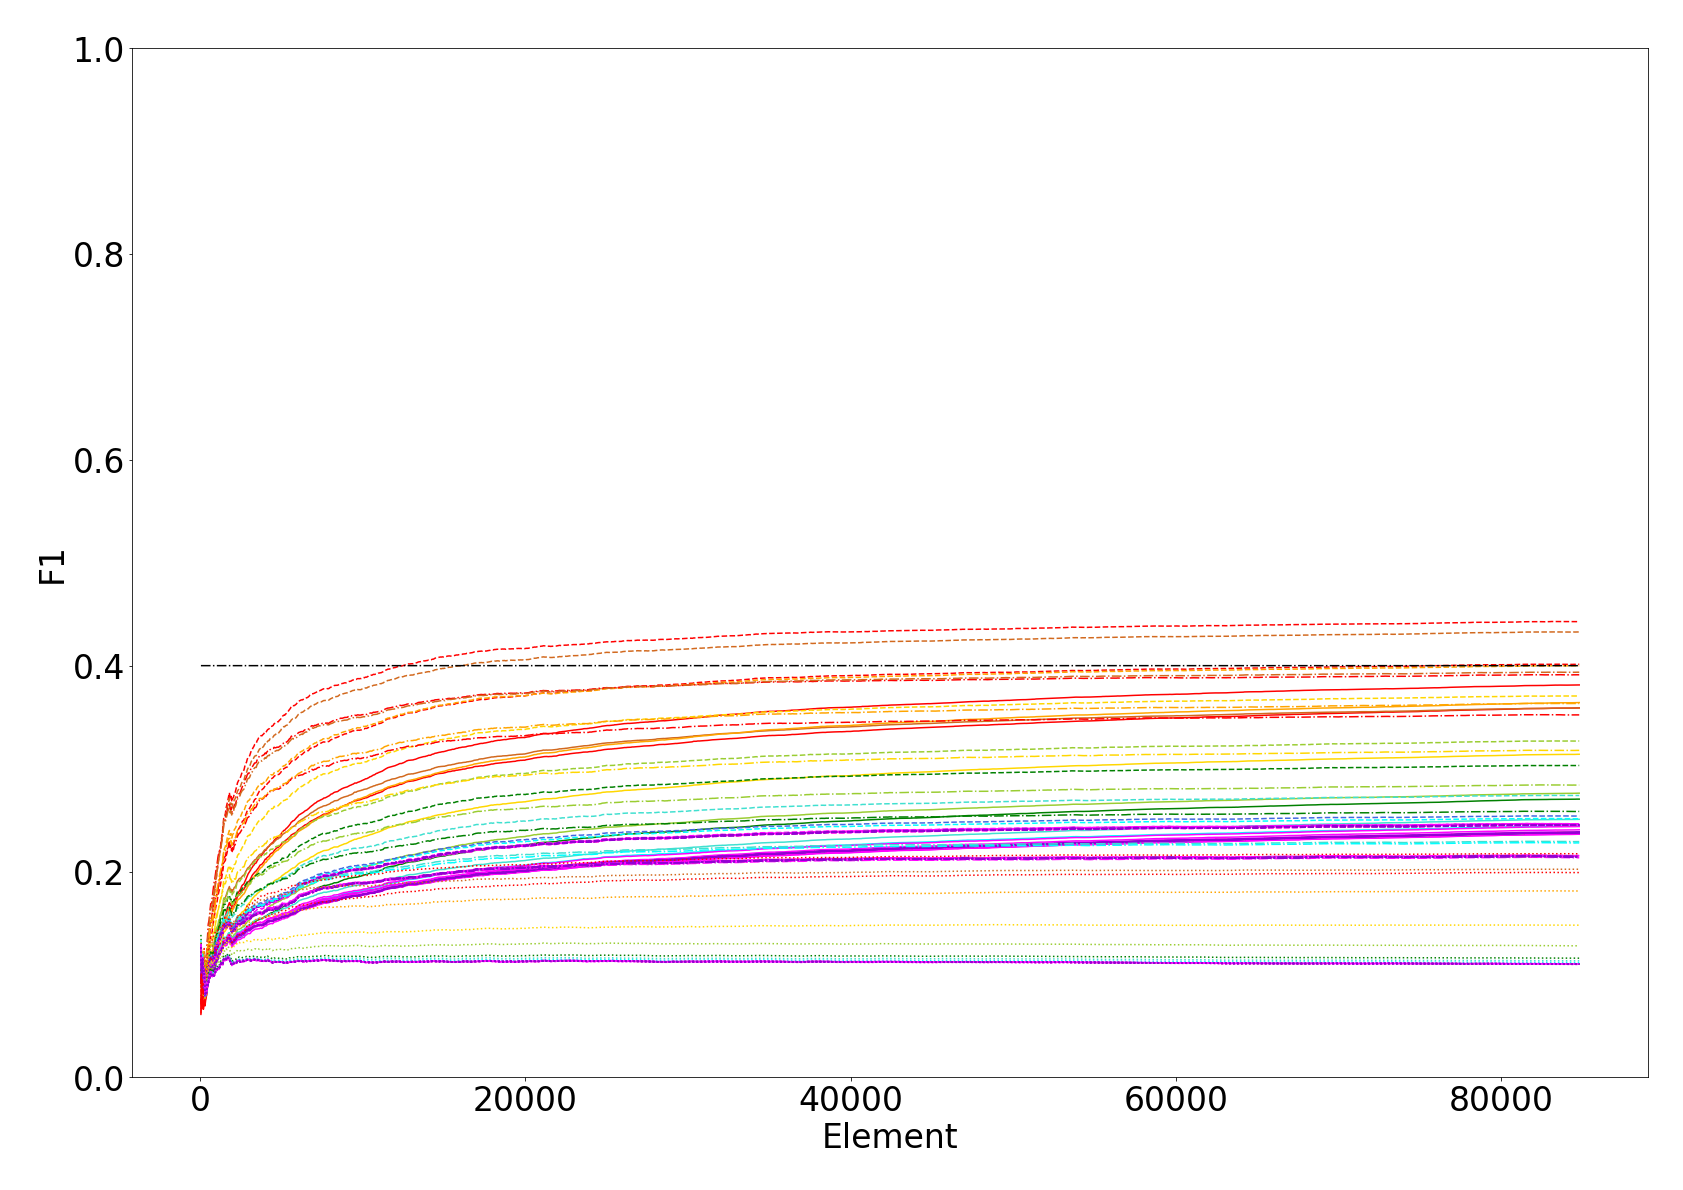
\includegraphics[width=\linewidth]{recofit_5_11.png}}
\caption{Using the Recofit dataset, the F1 Score in whole instrumentation with a memory limit of 3.0 MB. The horizontal dashed line represent the F1 score of kNN offline.}
\label{recofit}
\end{figure}
We observe the whole instrumentation is less stable in F1 score across all precisions. Moreover, gain in F1 score is significant in the case of very low precisions, precisely precisions between 2 and 5 inclusively. All tests are on the node instrumentation on all Banos 6 dataset randomizations tested give similar results.
In the case of the Recofit dataset, the gains in F1 score are even more important, going as far as to have a better F1 score than the reference offline KNN classifier.
\subsection{Reducing on exponents}
Table \ref{tab3} is the evaluation of the F1 score relative gain or loss using the node instrumentation on precision 52, with a focus on exponent reduction. Each measure is:
\begin{equation}
Gain = F1_{e=i} / F1_{e=11}-1 \label{eq2}
\end{equation}
measuring the relative gain or loss in F1-score compared to the equivalent model at exponent length 11.
\begin{table}[htbp]
\caption{Performance on exponent lengths}
\begin{center}
\begin{tabular}{|c|c|c|c|c|c|c|}
\hline
\textbf{Data}&\textbf{Mem}&\textbf{Tree}&\textbf{2}&\textbf{3}&\textbf{4}&\textbf{5}\\
\hline
Banos&0.6MB&1&0\%&-10.15\%&4.44\%&0\% \\
\cline{3-7}&&5&0\%&-2.88\%&0\%&-2.22\%\\
\cline{3-7}&&10&0\%&-3.19\%&2.22\%&2.22\% \\
\cline{3-7}&&50&0\%&-1.17\%&0\%&0\% \\
\cline{2-7}&3.0MB&1&0\%&-18.47\%&0\%&0\% \\
\cline{3-7}&&5&0\%&-6.31\%&0\%&0\% \\
\cline{3-7}&&10&0\%&-5.13\%&0\%&0\% \\
\cline{3-7}&&50&0\%&-2.79\%&0\%&0\% \\
\hline
Recofit&0.6MB&1&0\%&-70.47\%&-1.68\%&0\% \\
\cline{3-7}&&5&0\%&-68.72\%&-0.59\%&0\% \\
\cline{3-7}&&10&0\%&-65.56\%&-0.01\%&0\% \\
\cline{3-7}&&50&0\%&-40.86\%&0.02\%&0\% \\
\cline{2-7}&3.0MB&1&0\%&-72.87\%&-1.92\%&0\% \\
\cline{3-7}&&5&0\%&-75.39\%&-0.78\%&0\% \\
\cline{3-7}&&10&0\%&-75.07\%&-0.38\%&0\% \\
\cline{3-7}&&50&0\%&-66.73\%&-0.06\%&0\% \\
\hline
\end{tabular}
\label{tab3}
\end{center}
\end{table}

The F1 score does not significantly change as the exponent length is reduced up until length 2 for Banos and length 3 for Recofit where the F1 score drops. In the case of the whole instrumentation, the F1 scores are dropping even more critically in the case of exponent length 2 and 3, and in Recofit, exponent length 4 consistently give better performance from 2 to 4\%. Thus, the exponent 4 is the optimal limit of exponent reduction on both instrumentations.

\subsection{Expected gain}
Figure ??? is the evaluation of the F1 score on the model to evaluation optimal potential gains. We consider:
\begin{enumerate}
    \item 0.6MB of memory, uninstrumented,
    \item 1.2MB of memory, uninstrumented,
    \item 1.2MB of memory, node instrumented exponent 4 and precision 3,
    \item 1.2MB of memory, whole instrumented exponent 4 and precision 3.
\end{enumerate}
Each tree quantity is concurrently plotted. Consider the case where the performance needs to be improved at the same memory footprint: reducing the precision and using the space left for more nodes is the same process as the result shown. This graph constitutes a simulation of the potential performance gain obtained by this memory reduction: the first curves are the baseline performance, the theoretical upper bound to the performance gain of minimal memory footprint, the best node reduced obtainable performance and the best whole reduced obtainable performance.
%BANOS FIGURE: 52,1.0, 52,2.0, 2.0 node exponent 4 precision 3 (8 bits), 2.0 whole exponent 4 precision ? MOST COMPLEX PLOT
%RECOFIT FIGURE: 52,1.0, 52,2.0, 2.0 node exponent 4 precision 3 (8 bits), 2.0 whole exponent 4 precision ?
We observe here an improvement in F1 score of 9\% using double the memory space. As observed in the previous research \cite{khannouz2020benchmark}, a greater memory limit significantly improves the performance of the classifier. The minimal node curve is very close to the double memory curve, meaning significant memory is possible. Finally, the minimal whole approach better results to the double memory curve, meaning memory reduction can even significantly improve F1 score performance.
\section{Conclusions}
\subsection{Node instrumentation}
From our results, we see reducing the mantissa and the exponent length impacts negatively but insignificantly the F1 score down to and including length 3 and 4 respectively. Thus, with 1 bit for the sign, 4 bits for the exponent and 3 bits for the mantissa, our research proves the bound of the node of the Mondrian trees could be implemented using 8-bit Minifloats with minimal loss to F1 score.  Indeed, as alternative floating-point formats are growing in popularity, Minifloats may become an important part of machine learning optimization, and we see that opportunity in Mondrian forests in Human Activity Recognition. As our results are consistent with similar Human Activity Recognition datasets and random order variations, it suggest these results may be generalizable to most Human Activity Recognition tasks. Thus, the memory footprint can be greatly reduced through minimizing the size of nodes to bytes, but may require an involved and efficient implementation of byte-wise operations to fully harness the efficiency obtained by our results.
The insignificance of precision can be attributed to the randomness characteristic of Mondrian forests. Indeed, since the splits are already randomized, the node bounds do not need precision, as the error induced by a lack of precision is in most cases lesser or equal to the initial randomness of bounds.
This major reduction in memory occupied by nodes in Mondrian trees indicates Mondrian forests are potentially a state-of-the-art data streaming solution for Human Activity Recognition on smart objects.
\subsection{Whole instrumentation}
From our results, we see reducing the mantissa length impacts positively and significantly the F1 score down to and including length 3. Moreover, the exponent length impacts negatively but not significantly the F1 score down to and including length 4, with some exceptions.\footnote{Classifiers with 1 tree have significant loss at exponent 4.} Thus, with 1 bit for the sign, 3 bits for the exponent and 4 bits for the mantissa, results indicate the memory bound of all double-precision floating-point numbers in the OrpailleCC implementation is of 8-bits. They could be implemented using 8 bit Minifloats. Since precision reduction can significantly improve F1 score, variable-length operations should be considered, as even with a considerable memory loss, as lower precision in this instrumentation gives better performance.
The whole instrumentation difference in results can only be attributed to low precision hyperparameters, low precision splits or both. Since hyperparameters can be represented precisely with 4 bits, clearly low precision hyperparameters cannot be the cause of higher F1 score. Thus, we are left with the task of explaining why low precision splits improve the F1 score. We hypothesize low precision random splits may lower the complexity of the search space, since low precision transforms random choice to a stepwise function, forcing the algorithm to explore more equidistant splits. In other words, we believe this improvement is an optimization on the normally distributed splits implemented in Mondrian forests. Since this explanation is not based entirely on Human Activity Recognition, further research may prove this insight can be applied to other tasks and even other similar types of classifiers.
\subsection{Global}
Conclusions are ordered from precise to general.
\begin{enumerate}
\item For Mondrian forests on Human Activity Recognition tasks, it is clear nodes double-precision bounds could be reduced to byte-precision, while splits have an advantage to be calculated in variable-length precision under 16-bit. Improved implementations and further research are needed to ground this phenomenon in practice other Human Activity Recognition datasets.
\item For Mondrian forests, a major reduction in memory footprint as well as improvement in performance can be achieved through precision reduction. However, precision and exponent length may need to become adjustable hyperparameters to fully improve performance, which may make hyperparameter search significantly more complex.
\item For machine learning classifiers using normally distributed randomized choices, further research is needed to confirm or infirm if this improvement in F1 score is entirely caused by the reduction of the search space.
\end{enumerate}

\section*{Acknowledgment}

This work was made in continuous cooperation with Martin Khannouz and Yohan Châtelain. Computations were made with Compute Canada's resources. Most of this work was accomplished in the context of Concordia University's computer science honours project.

\bibliographystyle{ieeetr}
\bibliography{biblio.bib}

% \begin{thebibliography}{00}
% \bibitem{b2} M. Khannouz and T. Glatard, "A Benchmark of Data Stream Classification for Human Activity Recognition on Connected Objects," Sensors, vol. 20, no. 6486, 2020.
% \bibitem{b3} Y. Chatelain, Tools for debugging and optimizing floating point calculations in an HPC context, Paris: Université Paris-Saclay, 2019. 
% \bibitem{b4} E. Chung, J. Fowers, K. Ovtcharov, M. Papamichael, A. Caulfield, T. Massengill, M. Liu, D. Lo, S. Akalay and M. Haselman, "Serving dnns in real time at datacenter scale with project brainwave," IEEE Micro, vol. 38, no. 2, pp. 8-20, 2018.
% \bibitem{b5} J. L. Gustafson and I. T. Yonemoto, "Beating floating point at its own game : Posit arithmetic," Supercomputing Frontiers and Innovations, vol. 4, no. 2, pp. 71-86, 2017.
% \bibitem{b1} B. Lakshminarayanan, D. M. Roy and Y. T. Whye, "Mondrian Forests: Efficient Online Random Forests," Advances in Neural Information Processing Systems 27 (NIPS), vol. 1406, no. 2673, pp. 3140-3148, 2015.
% \bibitem{b6} C. Denis, P. d. O. Castro and E. Petit, "Verificarlo: checking floating point accuracy through Monte Carlo Arithmetic," in 2016 IEEE 23nd Symposium on Computer Arithmetic (ARITH), Silicon Valley, 2016.
% \bibitem{b7} A. Adje, D. B. Khalifa and M. Martel, Fast and Efficient Bit-Level Precision Tuning, Perpignan: Perpignan University, 2021. 
% \bibitem{b8} Y. Chatelain, E. Petit, P. d. O. Castro, G. Lartigue and D. Defour, "Automatic Exploration of Reduced Floating-Point Representations in Iterative Methods," in 25th International Conference Euro-Par 2019 Parallel Processing, Göttingen, 2020. 
% \bibitem{b9} O. Banos, M. A. Toth, M. Damas, H. Pomares and I. Rojas, "Dealing with the effects of sensor displacement in wearable activity recognition," Sensors, vol. 14, no. 6, pp. 9995-10023, 2014.
% \bibitem{b10} O. Banos, M. A. Toth, M. Damas, H. Pomares, I. Rojas and O. Amft, "A benchmark dataset to evaluate sensor displacement in activity recognition," in Proceedings of the 14th International Conference on Ubiquitous Computing (Ubicomp 2012), Pittsburgh, 2012. 
% \bibitem{b11} D. Morris, T. S. Saponas, A. Guillory and I. Kelner, "RecoFit: Using a Wearable Sensor to Find, Recognize, and Count Repetitive Exercises," in CHI '14 Proceedings of the SIGCHI Conference on Human Factors in Computing Systems, Toronto, 2014. 
% \end{thebibliography}
\vspace{12pt}

\end{document}
